% Asset ID: A21DifferentiationTikZ-001
% Source: Chapter 9 Differentiation transcript + slide evidence
% Related lesson section: Core Theory 3
% Purpose: Show tangent gradients on y = sin x at key points.
\documentclass[tikz,border=8pt]{standalone}
\usepackage{amsmath}
\usepackage{pgfplots}
\pgfplotsset{compat=1.18}
\begin{document}
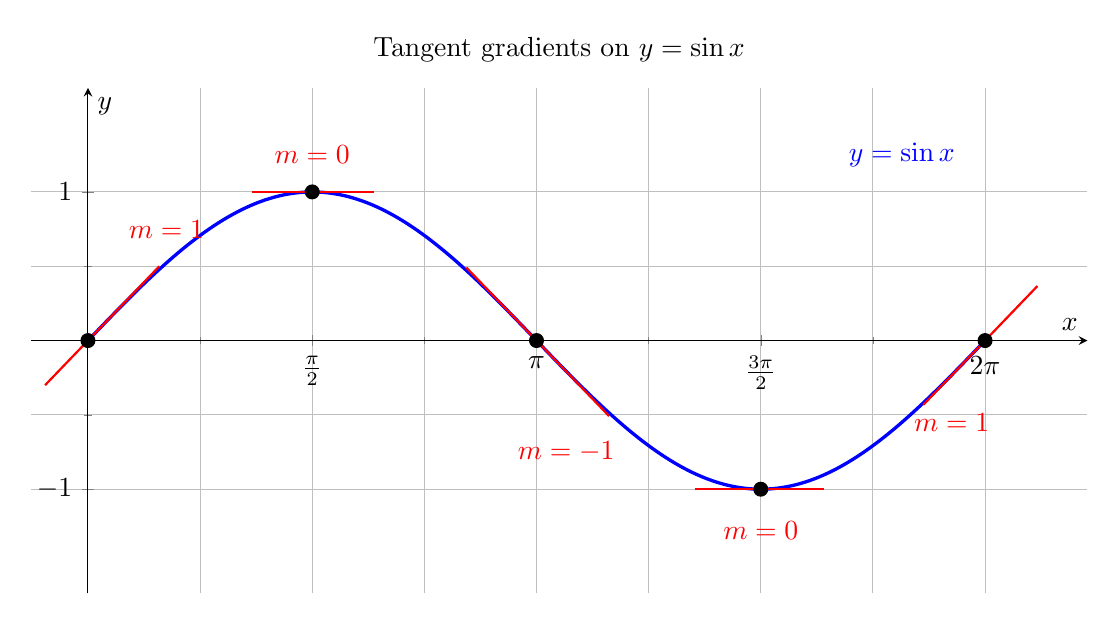
\begin{tikzpicture}
\begin{axis}[width=15cm,height=8cm,axis lines=middle,xmin=-0.4,xmax=7,ymin=-1.7,ymax=1.7,xtick={0,1.5708,3.1416,4.7124,6.2832},xticklabels={$0$,$\frac{\pi}{2}$,$\pi$,$\frac{3\pi}{2}$,$2\pi$},ytick={-1,0,1},xlabel={$x$},ylabel={$y$},title={Tangent gradients on \(y=\sin x\)},samples=200,domain=0:6.2832,grid=both,minor tick num=1]
\addplot[very thick, blue] {sin(deg(x))};
\node[blue] at (axis cs:5.7,1.25) {$y=\sin x$};
\addplot[red, thick, domain=-0.3:0.5] {x};
\node[red] at (axis cs:0.55,0.75) {$m=1$};
\addplot[red, thick, domain=1.15:2.0] {1};
\node[red] at (axis cs:1.5708,1.25) {$m=0$};
\addplot[red, thick, domain=2.65:3.65] {-(x-3.1416)};
\node[red] at (axis cs:3.35,-0.75) {$m=-1$};
\addplot[red, thick, domain=4.25:5.15] {-1};
\node[red] at (axis cs:4.7124,-1.28) {$m=0$};
\addplot[red, thick, domain=5.85:6.65] {x-6.2832};
\node[red] at (axis cs:6.05,-0.55) {$m=1$};
\addplot[only marks, mark=*, mark size=2.5pt] coordinates {(0,0)(1.5708,1)(3.1416,0)(4.7124,-1)(6.2832,0)};
\end{axis}
\end{tikzpicture}
\end{document}
